%%%%%%%%%%%%%%%%%%%%%%%%%%%%%%%%%%%%%%%%%%%%%%%%%%%%%%%%%%%%%%%%%%%%%%%%%%%%%%%%%%%%%%%%%%%%%%%%%%%
% Chapter 4 -> Experiments
% Author: Eduardo G Gusmao
%%%%%%%%%%%%%%%%%%%%%%%%%%%%%%%%%%%%%%%%%%%%%%%%%%%%%%%%%%%%%%%%%%%%%%%%%%%%%%%%%%%%%%%%%%%%%%%%%%%
\chapter{Experiments}
\label{cha:experiments}

\graphicspath{{chapter4/figs/}}

% Introduction
In this chapter, we define the experiment design of this study. Such experiment design is summarized in Figure~\ref{fig:gusmao_experiment_design_pipeline}. First, we describe all data sets and repositories used in this study (Section~\ref{sec:data.description}). Then, we show how the genomic signals used as input for our computational footprinting method were created and processed (Section~\ref{xxx}), following the theoretical basis described in Section~\ref{xxx}. After, we define the methodology used to train and apply our computational footprinting method (Section~\ref{xxx}), following the theoretical basis described in Section~\ref{xxx}. Furthermore, we discuss the methodologies we used to evaluate our computational footprinting approach and competing methods (Section~\ref{xxx}). Next, we define how each competing method was executed and which parameters were used (Section~\ref{sec:competing.methods}). Finally, we close this chapter with a brief discussion on the choice of such experimental design (Section~\ref{sec:discussion.4}).

% Figure - Experiment design
\begin{figure}[h!]
\centering
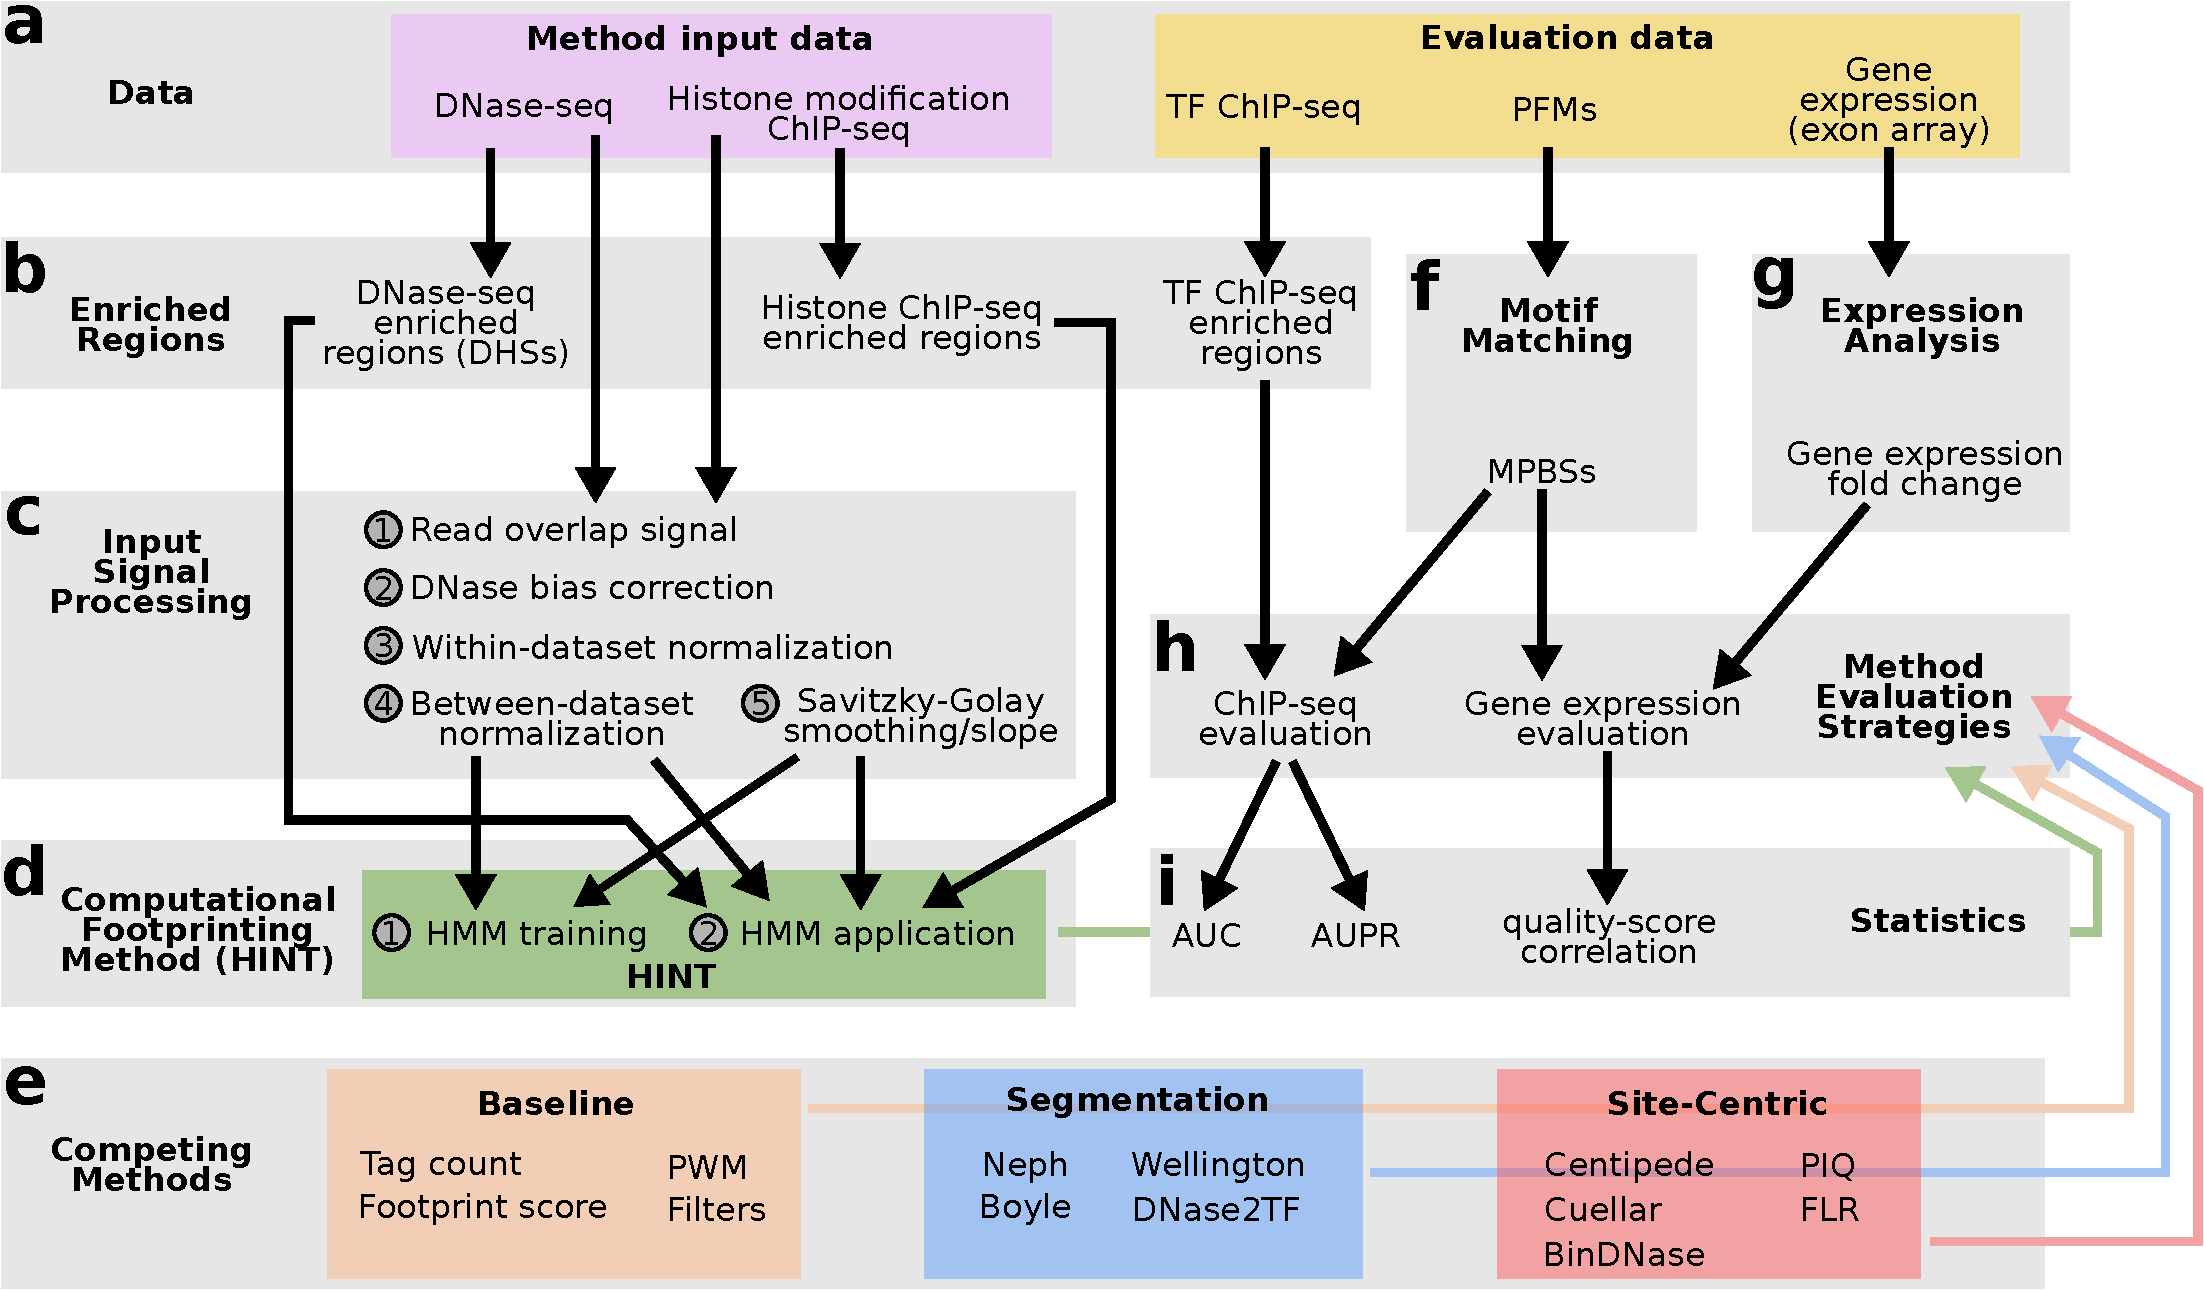
\includegraphics[width=0.99\textwidth]{gusmao_experiment_design_pipeline}
\caption[Experiment design]{\textbf{Experiment design.} (\textbf{a}) We categorize our data sets as: (1) method input data -- used as input for our computational footprinting method and competing methods and (2) evaluation data -- used to create the gold standard in which the computational footprinting methods are evaluated. The method input data includes DNase-seq and histone modification ChIP-seq. The evaluation data includes position frequency matrices (PFMs) and transcription factor (TF) ChIP-seq data. In both cases we also use the genome sequence as data input, which was not represented in this Figure for simplicity. (\textbf{b}) We process the method input data as described in the Section~\ref{xxx}. The signal processing pipeline consists of: (1) creating the genomic signal by evaluating the aligned read overlap; (2) correcting the DNase-seq signal for DNase~I experimental bias; (3) normalizing the signals using the within-dataset approach; (4) normalize the signals using the between-dataset approach and (5) create the slope signal by using the Savitzky-Golay smoothing filter approach. (\textbf{c}) Using the normalized and slope signals, we train and apply our computational footprinting method on particular genomic locations. (\textbf{d}) Given the footprint predictions resulting from the application of our method, we can evaluate the performance using two distinct approaches: (1) using motif-predicted binding sites (MPBSs) and TF ChIP-seq data and (2) using MPBSs and gene expression data. (\textbf{e}) In light of the evaluation methodologies, we compare our computational footprinting approach (HINT -- HMM-based identification of TF footprints; green box) with a number of competing methods (yellow, blue and red boxes).}
\label{fig:gusmao_experiment_design_pipeline}
\end{figure}

%%%%%%%%%%%%%%%%%%%%%%%%%%%%%%%%%%%%%%%%%%%%%%%%%%%%%%%%%%%%%%%%%%%%%
% Section: Data Description
%%%%%%%%%%%%%%%%%%%%%%%%%%%%%%%%%%%%%%%%%%%%%%%%%%%%%%%%%%%%%%%%%%%%%
\section{Data Description}
\label{sec:data.description}

% Introduction
In this section we describe the data sources for this project. We state where we obtained data used: (1) as input for the computational footprinting approach (Section~\ref{sec:method.input.data}); (2) as input for the creation of the evaluation gold standard data sets (Section~\ref{sec:evaluation.data}); and (3) as extra input for competing methods (Section~\ref{sec:competing.methods.additional.data}).

% Further notes
All experimental organism-specific data (DNase-seq, ChIP-seq and gene expression) are based on the human genome build 37 (hg19), except the DNase-seq for m3134 cell and ChIP-seq for the GR transcription factor, which were based on mouse genome build 37 (mm9). Chromosome~Y was removed from all analyses. The genomic sequences (DNA) were obtained in ENCODE~\cite{encode2012}.

%%%%%%%%%%%%%%%%%%%%%%%%%%%%%%%%%%%%%%%%%%%%%%%%%%%%%%%%%%%%%%%%%%%%%
% Section: Method Input Data
%%%%%%%%%%%%%%%%%%%%%%%%%%%%%%%%%%%%%%%%%%%%%%%%%%%%%%%%%%%%%%%%%%%%%
\subsection{Method Input Data}
\label{sec:method.input.data}

% DNase-seq
DNase-seq aligned reads were obtained from ENCODE~\cite{encode2012}. To perform the computational footprint experiments, we obtained data regarding cell types H1-hESC, HeLa-S3, HepG2, Huvec, K562, LNCaP and MCF-7 from Crawford's Lab at Duke University (labeled with the initials of their institution ``DU'') and cell types H7-hESC, HepG2, Huvec, K562 and m3134 from Stamatoyannopoulous' lab at University of Washington (labeled with the initials of their institution ``UW''). We also used deproteinized DNase-seq experiments from cell types MCF-7 and K562 (Crawford lab)~\cite{yardimci2014} and IMR90 (Stamatoyannopoulous lab)~\cite{lazarovici2013}. DNase-seq experiments labeled with ``DU'' follow the single-hit protocol, while the experiments labeled with ``UW'' follow the double-hit protocol. In addition, to perform the DNase-seq bias estimation clustering, we used all cell types from ENCODE's Tier 1 and Tier 2 cell types, generated in Crawford's and Stamatoyannopoulous' labs. See Supplementary Table~\ref{tab:dataencode.dnase} for a full DNase-seq data description and accession numbers.

% Histone modifications ChIP-seq
Histone modifications ChIP-seq aligned reads were obtained from ENCODE~\cite{encode2012}. It was obtained data regarding cell types H1-hESC, HeLa-S3, HepG2 and K562 and histone modifications H3K4me1, H3K4me3, H3K9ac, H3K27ac and H2A.Z generated at the Broad Institute and in the Bernstein's lab at the Massachusetts General Hospital/Harvard Medical School. See Supplementary Table~\ref{tab:dataencode.histone} for a full histone modification ChIP-seq data description and accession numbers.

%%%%%%%%%%%%%%%%%%%%%%%%%%%%%%%%%%%%%%%%%%%%%%%%%%%%%%%%%%%%%%%%%%%%%
% Section: Evaluation Data
%%%%%%%%%%%%%%%%%%%%%%%%%%%%%%%%%%%%%%%%%%%%%%%%%%%%%%%%%%%%%%%%%%%%%
\subsection{Evaluation Data}
\label{sec:evaluation.data}

% TF ChIP-seq
Transcription factor (TF) ChIP-seq enriched regions (peaks and summits) were obtained in ENCODE Analysis Working Group (AWG) track with exception of the following experiments, in which the enriched regions were obtained using bowtie-2~\cite{langmead2012} and MACS~\cite{zhang2008}: (1) AR (R1881 treatment) ChIP-seq raw sequences for LNCaP cell type was obtained in gene expression omnibus (GEO) with accession number GSM353644~\cite{yu2010}; (2) ER (40 and 160 minutes after estradiol treatment) ChIP-seq raw sequences for MCF-7 cell type was obtained in GEO with accession number GSE54855~\cite{guertin2014}; (3) GR (dexamethasone treatment) ChIP-seq raw sequences for m3134 cell type was obtained in the sequence read archive (SRA) under study number SRP004871~\cite{john2011}. See Supplementary Table~\ref{tab:dataencode.pfm.chipseq} for a full TF ChIP-seq data description and accession numbers. This table contains information on TF ChIP-seq data and also on the PFMs associated to these TF ChIP-seq dataset for the TF ChIP-seq evaluation scenario (more details on Section~\ref{sec:chipseq.evaluation}).

% Gene expression data
Expression profiling by array (Affymetrix Human Exon 1.0 ST Array) data was obtained directly from GEO. It was downloaded data for cell types H1-hESC, K562 and GM12878 generated in the Microarray Core from the Center for Functional Genomics in SUNY-University at Albany. All samples from each cell type was used to infer the overall gene expression profile. See Supplementary Table~\ref{tab:data.expression} for a full gene expression data description and accession numbers.

% PFMs
TF motifs (PFMs) were obtained from the repositories Jaspar~\cite{mathelier2014}, Uniprobe~\cite{robasky2011} and Transfac~\cite{matys2006}. These non-organism-specific data (PFMs) were obtained for the subphylum \emph{Vertebrata}. \emph{De novo} PFMs 0458 and 0500 were downloaded from Neph et al.~\cite{neph2012a}. See Supplementary Tables~\ref{tab:dataencode.pfm.chipseq} and~\ref{tab:dataencode.pfm.flrexp} for a full description on the PFMs used in this work and their IDs within their respective repositories.

%%%%%%%%%%%%%%%%%%%%%%%%%%%%%%%%%%%%%%%%%%%%%%%%%%%%%%%%%%%%%%%%%%%%%
% Section: Competing Methods Additional Data
%%%%%%%%%%%%%%%%%%%%%%%%%%%%%%%%%%%%%%%%%%%%%%%%%%%%%%%%%%%%%%%%%%%%%
\subsection{Competing Methods Additional Data}
\label{sec:competing.methods.additional.data}

% Genomic data
Additionally, to create the genomic data input for the method Centipede, we obtained PhastCons conservation score (placental mammals on the 46-way multiple alignment)~\cite{siepel2005} and Ensembl gene annotation from ENCODE~\cite{hubbard2002}. 

%%%%%%%%%%%%%%%%%%%%%%%%%%%%%%%%%%%%%%%%%%%%%%%%%%%%%%%%%%%%%%%%%%%%%
% Section: Signal Creation and Processing
%%%%%%%%%%%%%%%%%%%%%%%%%%%%%%%%%%%%%%%%%%%%%%%%%%%%%%%%%%%%%%%%%%%%%
\section{Signal Creation and Processing}
\label{sec:signal.creation.processing}

% Introduction
In this section we describe the generation of the DNase-seq signal and histone modification ChIP-seq signal used as input for our computational footprinting method. For that, we use a pipeline which consists on: (1) raw signal creation and pre-processing (Section~\ref{sec:raw.signal.creation.preprocessing}); (2) correction of the DNase-seq signal for experimental artifacts (Section~\ref{sec:dnase.experimental.bias.correction}) and (3) normalization, smoothing and slope calculation (Section~\ref{sec:normalization.smoothing.slope}).

%%%%%%%%%%%%%%%%%%%%%%%%%%%%%%%%%%%%%%%%%%%%%%%%%%%%%%%%%%%%%%%%%%%%%
% Section: Raw Signal Creation and Pre-Processing
%%%%%%%%%%%%%%%%%%%%%%%%%%%%%%%%%%%%%%%%%%%%%%%%%%%%%%%%%%%%%%%%%%%%%
\subsection{Raw Signal Creation and Pre-Processing}
\label{sec:raw.signal.creation.preprocessing}

% Introduction
As described in Section~\ref{sec:ngs.methods}, we are able to create a genome-wide signal from NGS-based experiments. In a brief recapitulation, the NGS-based experiments produces short DNA fragments (termed ``reads'') which are mapped into the genome using an alignment software such as Bowtie~2~\cite{langmead2012} or the Burrows-Wheeler Aligner (BWA)~\cite{li2009b}. Given these aligned reads, we are able to create a time series-like signal in which the $x$-axis represents the genomic coordinates (also referred to as genomic positions), i.e. each nucleotide of the DNA sequence represents a genomic position; and the $y$-axis represents the signal intensity, i.e. the number of reads aligned to the genomic positions.

% DNase-seq signal
The raw DNase-seq signal (also referred to as DNase-seq counts or DNase-seq tag counts) is created by counting, for every genomic position, the number of overlapping read's $5^\prime$ position (i.e., the ``start'' of the read). We only consider the $5^\prime$ because that is the exact location in which the DNase I enzyme has nicked the DNA. For this reason, we can consider the DNase-seq signal as containing the maximum resolution possible (resolution at the base pair level).

% ChIP-seq signal
The raw histone modification ChIP-seq signal is created by counting, for every genomic position, the number of overlapping reads, after extending all reads (towards the $5^\prime \rightarrow 3^\prime$ direction), which are usually $20--36$ bp in length, to a total length of $200$ bp. The rationale behind the extension is that, when the immunoprecipitated fragments are recovered, the protein of interest (in this case, the modified histones) can be at any position inside the fragment. Since these fragments are, in average, $200$ bp in length, we perform the extension in order to cover all possible target-protein locations. For this reason, we can consider the ChIP-seq signal as having a much lower resolution than the DNase-seq signal, which translates to a more ``smoothed'' ChIP-seq signal in comparison to the sharp peaks of the DNase-seq signal.

% Raw signal pre-processing for experimental artifacts
Both DNase-seq and histone modification ChIP-seq signals are pre-processed using the state-of-the-art standard approaches~\cite{li2009a,li2011a}. Such pre-processing is needed in order to remove experimental artifacts. The pre-processing pipeline was performed using SAMtools~\cite{li2009a} and regards the following operations:
\vspace{0.2cm}
\noindent
\textbf{1.} Filter reads which are mapped to: (\textbf{a}) unassembled regions; (\textbf{b}) low-mappability regions as defined by Derrien et al.~\cite{derrien2012}; (\textbf{c}) the same exact genomic coordinate for more than four times as defined by Boyle et al.~\cite{boyle2011}.
\noindent
\textbf{2.} Correction of mapped reads for the underlying frequencies of nucleotides in the genome, since sequencing technologies tend to favor the sequencing of reads falling into CG-rich regions, i.e. regions with high content of the nucleotide C and G. The correction followed the work by Ashoor et al.~\cite{ashoor2013}.
\noindent
\textbf{3.} Correction of experimental artifacts using input-DNA, i.e. sequencing of the genome with all steps of the DNase-seq and ChIP-seq protocol except for the DNase~I digestion (DNase-seq) and target protein immunoprecipitation (ChIP-seq). Such data set can be regarded as a biological ``control'' data set. Such correction was based on Diaz et al.~\cite{diaz2012}.
\vspace{0.2cm}

%%%%%%%%%%%%%%%%%%%%%%%%%%%%%%%%%%%%%%%%%%%%%%%%%%%%%%%%%%%%%%%%%%%%%
% Section: DNase-seq Experimental Bias Correction
%%%%%%%%%%%%%%%%%%%%%%%%%%%%%%%%%%%%%%%%%%%%%%%%%%%%%%%%%%%%%%%%%%%%%
\subsection{DNase-seq Experimental Bias Correction}
\label{sec:dnase.experimental.bias.correction}

% TODO

%%%%%%%%%%%%%%%%%%%%%%%%%%%%%%%%%%%%%%%%%%%%%%%%%%%%%%%%%%%%%%%%%%%%%
% Section: Normalization, Smoothing and Slope
%%%%%%%%%%%%%%%%%%%%%%%%%%%%%%%%%%%%%%%%%%%%%%%%%%%%%%%%%%%%%%%%%%%%%
\subsection{Normalization, Smoothing and Slope}
\label{sec:normalization.smoothing.slope}

% TODO

% TODO - Different scaling methodologies
Although the first normalization step (within-dataset) is always used in a local fashion~\cite{boyle2011}, the second normalization step, i.e. the scaling procedure, can be performed using either local or global values of the standard deviation and percentile. The local method is depicted in Equation~\ref{xxx}, using the same windowing as the normalization procedure. The global method consists on using a single estimate of standard deviation and percentile for each cell type.

%%%%%%%%%%%%%%%%%%%%%%%%%%%%%%%%%%%%%%%%%%%%%%%%%%%%%%%%%%%%%%%%%%%%%
% Section: Method Training and Application
%%%%%%%%%%%%%%%%%%%%%%%%%%%%%%%%%%%%%%%%%%%%%%%%%%%%%%%%%%%%%%%%%%%%%
\section{Method Training and Application}
\label{sec:method.training.application}

% Introduction
In this section we describe the methodology we used to train our computational footprinting method (Section~\ref{sec:method.training}) and apply such model to obtain footprint predictions (Section~\ref{sec:method.application}).

%%%%%%%%%%%%%%%%%%%%%%%%%%%%%%%%%%%%%%%%%%%%%%%%%%%%%%%%%%%%%%%%%%%%%
% Section: Method Training
%%%%%%%%%%%%%%%%%%%%%%%%%%%%%%%%%%%%%%%%%%%%%%%%%%%%%%%%%%%%%%%%%%%%%
\subsection{Method Training}
\label{sec:method.training}

% TODO

%%%%%%%%%%%%%%%%%%%%%%%%%%%%%%%%%%%%%%%%%%%%%%%%%%%%%%%%%%%%%%%%%%%%%
% Section: Method Application
%%%%%%%%%%%%%%%%%%%%%%%%%%%%%%%%%%%%%%%%%%%%%%%%%%%%%%%%%%%%%%%%%%%%%
\subsection{Method Application}
\label{sec:method.application}

% TODO

%%%%%%%%%%%%%%%%%%%%%%%%%%%%%%%%%%%%%%%%%%%%%%%%%%%%%%%%%%%%%%%%%%%%%
% Section: Method Evaluation Strategies
%%%%%%%%%%%%%%%%%%%%%%%%%%%%%%%%%%%%%%%%%%%%%%%%%%%%%%%%%%%%%%%%%%%%%
\section{Method Evaluation Strategies}
\label{sec:method.evaluation.strategies}

% Introduction
In this section we discuss the methodology used to evalute the footprint predictions from our method and competing methods. We used two evaluation approaches. The first is based on ChIP-seq data (ChIP-seq evaluation) and the second is based on gene expression data (gene expression evaluation).

% This section
We start this section by defining how we obtained motif-predicted binding sites (MPBSs) by performing a string-matching algorithm (Section~\ref{sec:mpbs}). Such MPBSs are required for both evaluation strategies. Next, we define a interval-based algebra (Section~\ref{sec:interval.based.algebra}), which allows us to formally describe the evaluation methodologies. Finally, we describe the ChIP-seq evaluation methodology (Section~\ref{sec:chipseq.evaluation}) and the gene expression evaluation methodology (Section~\ref{sec:gene.expression.evaluation}).

%%%%%%%%%%%%%%%%%%%%%%%%%%%%%%%%%%%%%%%%%%%%%%%%%%%%%%%%%%%%%%%%%%%%%
% Section: Motif-Predicted Binding Sites (MPBSs)
%%%%%%%%%%%%%%%%%%%%%%%%%%%%%%%%%%%%%%%%%%%%%%%%%%%%%%%%%%%%%%%%%%%%%
\subsection{Motif-Predicted Binding Sites (MPBSs)}
\label{sec:mpbs}

All PFMs (see Supplementary Tables~\ref{tab:dataencode.pfm.chipseq} and~\ref{tab:dataencode.pfm.flrexp}) were converted into PWMs using the process described in Section~\ref{sec:mpbs}. This procedure was performed using Biopython~\cite{cock2009}. Also, we performed the background nucleotide frequency correction~\cite{stormo2000} and used a pseudocount of $0.1$ for all PFMs~\cite{boyle2011}.

Then, we created MPBSs by matching all PWMs against the human (hg19) and mouse (mm9) genomes using the fast performance motif matching tool MOODS~\cite{korhonen2009}. This procedure produces ``PWM bit-scores'' for every match. We determined a bit-score cutoff threshold by applying the dynamic programming approach described in~\cite{wilczynski2009} with a false positive rate (FPR) of $10^{-4}$.

% TODO XXX
% Move motif matching section here

%%%%%%%%%%%%%%%%%%%%%%%%%%%%%%%%%%%%%%%%%%%%%%%%%%%%%%%%%%%%%%%%%%%%%
% Section: Interval-Based Algebra
%%%%%%%%%%%%%%%%%%%%%%%%%%%%%%%%%%%%%%%%%%%%%%%%%%%%%%%%%%%%%%%%%%%%%
\subsection{Interval-Based Algebra}
\label{sec:interval.based.algebra}

% TODO XXX

%%%%%%%%%%%%%%%%%%%%%%%%%%%%%%%%%%%%%%%%%%%%%%%%%%%%%%%%%%%%%%%%%%%%%
% Section: ChIP-seq Evaluation
%%%%%%%%%%%%%%%%%%%%%%%%%%%%%%%%%%%%%%%%%%%%%%%%%%%%%%%%%%%%%%%%%%%%%
\subsection{ChIP-seq Evaluation}
\label{sec:chipseq.evaluation}

% Introduction
There is no well defined gold standard for the evaluation of footprinting methods. All works so far have used ChIP-seq of TFs in conjunction with motif-based predictions as ground truth. Although this method has some intrinsic biases, which will be stated in Section~\ref{sec:gene.expression.evaluation}, it provides a straightforward scenario for the evaluation of computational footprinting methods.

% Procedure
This evaluation procedure uses ChIP-seq experiments for the TFs being tested as experimental evidence of binding. These are simply the enriched regions (or peaks) based on the uniform processing of ENCODE Analysis Working Group (AWG) data track. In this evaluation scheme, MPBSs with ChIP-seq evidence (located within $100$ bp from the ChIP-seq peak summit) are considered ``true'' TFBSs; while MPBSs without ChIP-seq evidence are considered ``false'' TFBSs. Every TF prediction that overlaps a true TFBS is considered a correct prediction (true positive -- TP) and every prediction that overlaps with a false TFBS is considered an incorrect prediction (false positive -- FP). Therefore, true negatives (TN) and false negatives (FN) are, respectively, false and true TFBSs without overlapping predictions.

% ROC curves and AUC
The contingency table (TPs, FPs, TNs and FNs) enables us to create ROC curves, which describe the sensitivity (recall) increase as we decrease the specificity of the method. The area under the ROC curve (AUC) metric was evaluated at $1\%$, $10\%$ and $100\%$ false positive rates (FPR). By evaluating the AUC at different FPRs we can avoid misleading interpretations due to the rate in which the specificity decreases with sensitivity increase. The contingency table also enables us to evaluate the area under the precision-recall curve (AUPR). This metric is indicated for problems with imbalanced data sets (distinct number of positive and negative examples)~\cite{davis2006,fawcett2006}. In summary, this evaluation methodology provides four performance statistics for each TF: (1) AUC at $1\%$ FPR; (2) AUC at $10\%$ FPR; (3) AUC at $100\%$ FPR; and (4) AUPR. For any of these statistics, higher values indicate higher method performance. This evaluation procedure is schematized in Figure~\ref{fig:gusmao_chipseq_evaluation}

% TODO
% ChIP-seq evaluation figure
\begin{figure}[h!]
\centering
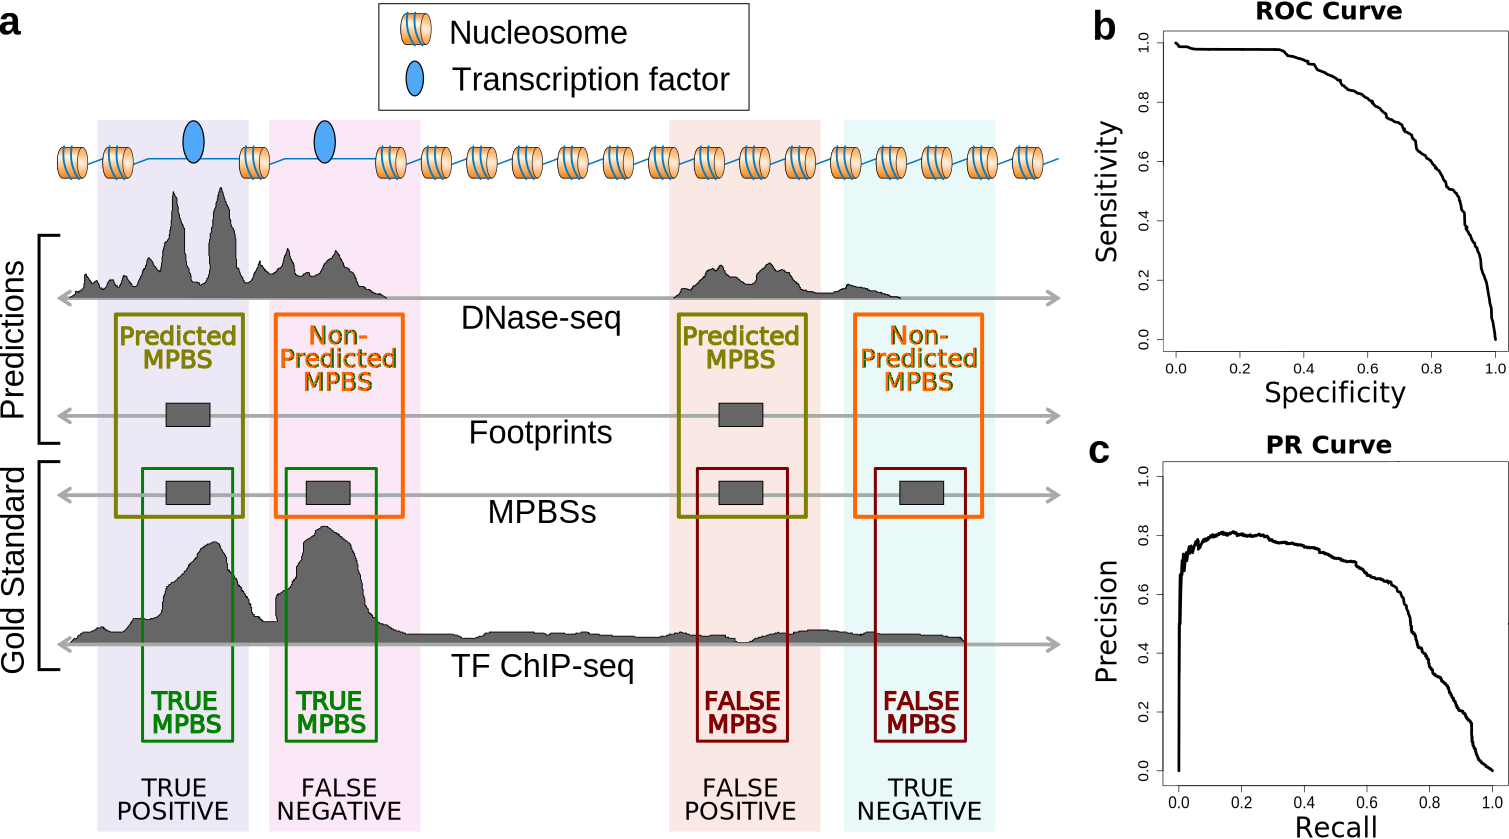
\includegraphics[width=0.99\textwidth]{gusmao_chipseq_evaluation}
\caption[ChIP-seq evaluation methodology]{\textbf{ChIP-seq evaluation methodology.} (\textbf{a}) Placeholder.}
\label{fig:gusmao_chipseq_evaluation}
\end{figure}

% TF Filtering
We filtered the TFs used in this approach in two ways: (1) The first approach consists on using data from Factorbook~\cite{wang2013} to disregard TF ChIP-seq data with a weak DNA motif landscape, which would mislead the interpretation of the results from this evaluation methodology. We considered only the TFs in which the top enriched motif from Factorbook's \emph{de novo} motif analysis was present in at least $300$ of the $500$ top-scored ChIP-seq peaks. (2) We filtered out all TFs in which less than $10\%$ of ChIP-seq peaks contained at least one MPBS associated. This approach filters MPBS results that did not work properly mainly due to PFMs with low conserved regions. The Supplementary Table~\ref{tab:dataencode.pfm.chipseq} shows information regarding each TF's PFM and ChIP-seq data set used. It also provides statistics, for each TF, on the number of ChIP-seq peaks, number of MPBSs and the proportion of ChIP-seq peaks which presented at least one MPBS.

% Evaluation scenarios
Different experiments required a different number of TFs being evaluated. Therefore, we created three ChIP-seq evaluation scenarios, described below.

\noindent{{\tt He Dataset:}} To replicate some analyses performed by He et al.~\cite{he2014}, we analyzed DNase-seq from cell types K562 (UW), LNCaP (DU) and m3134 (UW) on 36 TFs and we only evaluated the methods PWM, FS, TC, HINT, HINT-BC and HINT-BCN.

\noindent{{\tt Benchmarking Dataset:}} For comparative analysis of several competing methods, we selected the two cell types with highest number of TF ChIP-seq data sets evaluated in our study: K562(DU) with 59 TFs and H1hesc(DU) with 29 TFs. This was required due to the high computational demands of the execution of some competing methods. All methods described in this study were executed under this evaluation scenario.

\noindent{{\tt Comprehensive dataset:}} We have compiled a comprehensive data set containing 233 combinations of cells and TFs with matching cellular background. This data set was built from a catalog of 144 TF ChIP-seq and 13 DNase-seq data sets. This data is used to in analyses which require a large data set for statistical significance. In this scenario we only evaluated the methods PWM, FS, TC, HINT, HINT-BC and HINT-BCN.

% TODO
% formally (mathematically) define the procedure of creating this evaluation data set

%%%%%%%%%%%%%%%%%%%%%%%%%%%%%%%%%%%%%%%%%%%%%%%%%%%%%%%%%%%%%%%%%%%%%
% Section: Gene Expression Evaluation
%%%%%%%%%%%%%%%%%%%%%%%%%%%%%%%%%%%%%%%%%%%%%%%%%%%%%%%%%%%%%%%%%%%%%
\subsection{Gene Expression Evaluation}
\label{sec:gene.expression.evaluation}

% Introduction
The ChIP-seq evaluation approach requires TF ChIP-seq experiments which, as indicated by Yard{\i}mc{\i} et al.\cite{yardimci2014}, has some intrinsic biases. First, TF ChIP-seq peaks are also observed in indirect binding events. Second, they have a lower spatial resolution than DNase-seq. Therefore, false TFBSs might be regarded as true TFBSs by proximity to a real TFBS of a distinct TF. Recently, Yard{\i}mc{\i} et al.\cite{yardimci2014} indicated that footprint quality scores, as measured by the footprint likelihood ratio (FLR), were significantly higher in cells where the TF was expressed. This observation indicates that comparing changes in expression and quality of footprints in a pairs of cells could provide an alternative footprint evaluation measure. This led us to the development of a novel evaluation methodology termed FLR-Exp.

% Expression and MPBSs
We used limma~\cite{ritchie2015} to perform between-array normalization on expression of H1-hESC, K562 and GM12878 cells and obtain fold change estimates. Then, we retrieved all non-redudant PFMs from Jaspar in which gene symbol is a perfect match with genes present in the array platform. This leads us to 143 PFMs (see Supplementary Table~\ref{tab:dataencode.pfm.flrexp}). We applied a genome-wide motif matching (see Section~\ref{sec:mpbs}) using these PFMs to create MPBSs.

% Process
Afterwards, we evaluated the FLR score (Section~\ref{sec:xxx}), TC (Section~\ref{sec:xxx}) and FS (Section~\ref{sec:xxx}) for the footprints for each of the evaluated method, which intersects with MPBSs of a particular motif. We only considered the footprints within DHSs that are in common between the cell type pair being evaluated, as described in Yard{\i}mc{\i} et al.~\cite{yardimci2014}. We expect that TFs expressed in cell type A would present higher values regarding these metrics (FLR, TC and FS) with DNase-seq from cell type A in comparisson with these metrics evaluated with DNase-seq from cell type B, and vice-versa. We used a two-sample Kolmogorov-Smirnov (KS) test to assess the difference between each metrics' distribution between the two cell types being evaluated. The KS statistic, which varies from 0 to 1, is used to indicate the difference between two distributions; higher values indicate higher differences. As the KS score do not indicate the direction of the changes in distribution, we obtained a signed version by multiplying KS statistic by $-1$, in cases where the median of A $<$ median of B. We calculate the Spearman correlation between the signed KS test statistic and the expression fold change for each TF. Positive values indicate an association between expression of TFs and quality of footprint predictions. We will call this correlation ``FLR-Exp''. See Figure~\ref{sec:gusmao_flrexp_evaluation} for a graphical description of the method.

% TODO
% FLR-Exp evaluation figure
\begin{figure}[h!]
\centering
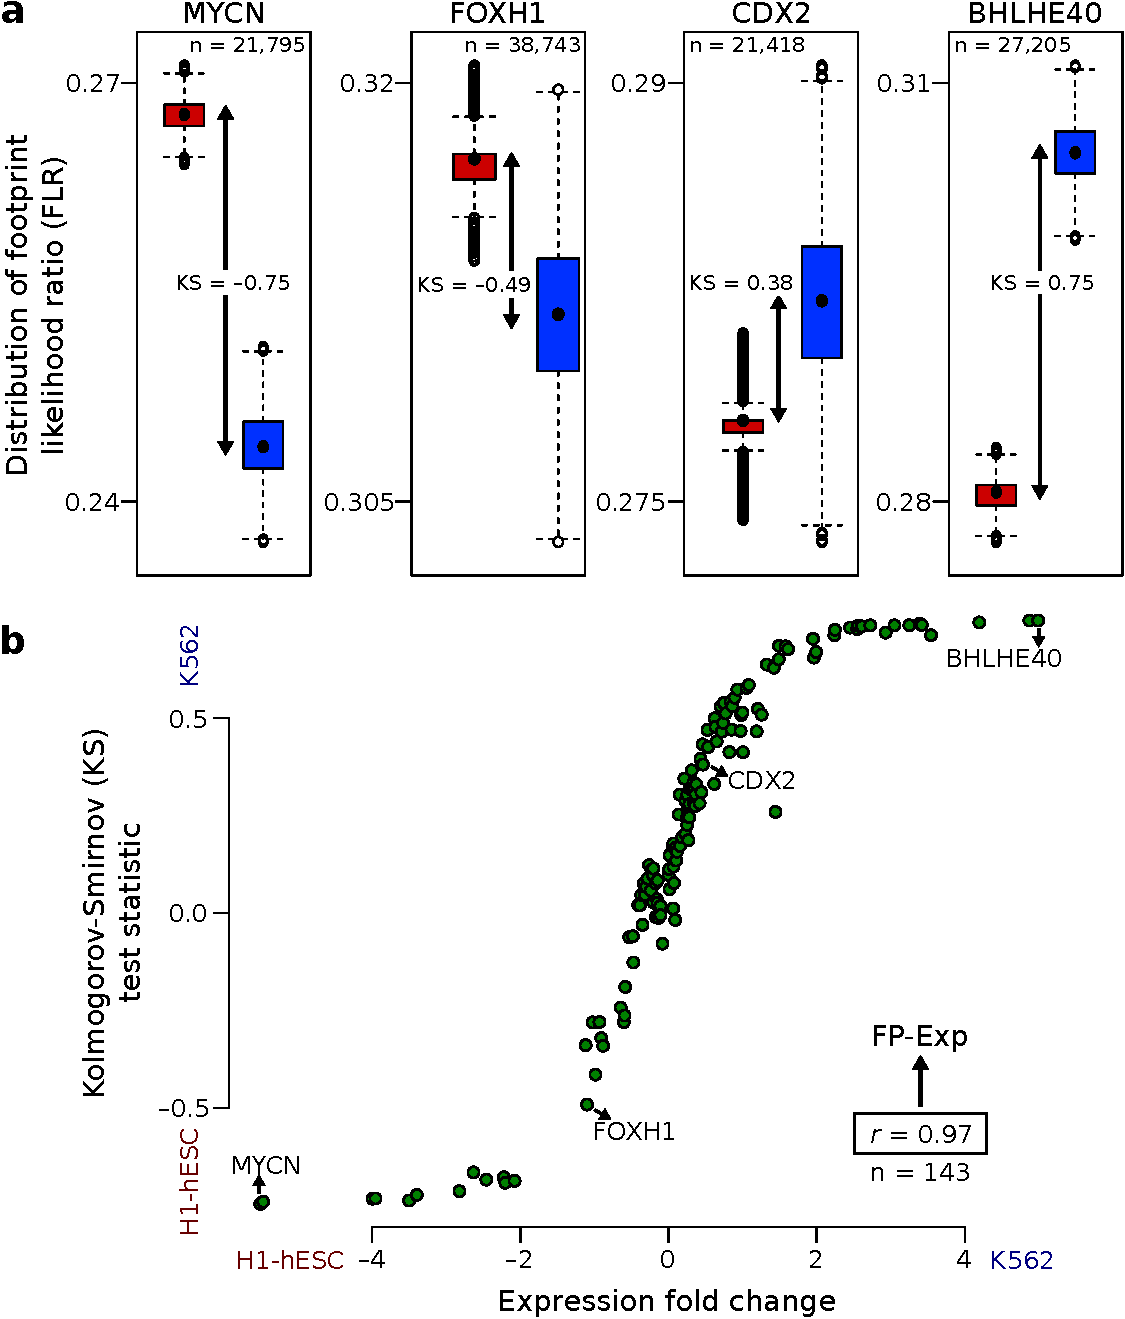
\includegraphics[width=0.99\textwidth]{gusmao_flrexp_evaluation}
\caption[FLR-exp evaluation methodology]{\textbf{FLR-exp evaluation methodology.} (\textbf{a}) Placeholder.}
\label{fig:gusmao_flrexp_evaluation}
\end{figure}

% TODO
% formally (mathematically) define the procedure of creating this evaluation data set

%%%%%%%%%%%%%%%%%%%%%%%%%%%%%%%%%%%%%%%%%%%%%%%%%%%%%%%%%%%%%%%%%%%%%
% Section: Competing Methods
%%%%%%%%%%%%%%%%%%%%%%%%%%%%%%%%%%%%%%%%%%%%%%%%%%%%%%%%%%%%%%%%%%%%%
\section{Competing Methods}
\label{sec:competing.methods}

% Introduction
In this section we present the full descpription of the parameterization and execution of competing methods. The competing methods are categorized as segmentation methods (Neph~\cite{neph2012a}, Boyle~\cite{boyle2011}, Wellington~\cite{piper2013} and DNase2TF~\cite{sung2014}) and site-centric methods (Centipede~\cite{pique2011}, Cuellar~\cite{cuellar2012}, PIQ~\cite{sherwood2014}, FLR~\cite{yardimci2014} and BinDNase~\cite{kahara2015}). Moreover, we also used baseline methods which correspond to simple computational footprinting approaches (PWM-Rank~\cite{gusmao2014}, FS-Rank~\cite{neph2012a,he2014}, TC-Rank~\cite{cuelar2012,he2014}, and signal processing filters). Computational resources necessary for the execution of segmentation and site-centric competing methods are summarized in Supplementary Table~\ref{tab:comp.resource}.

% Computational resources to execute methods
\begin{table}[h]
\begin{center}
\caption{Summary of computational resources. All methods were run in a Xeon E7-4870 40 CPU (2.4GHz per core). The figures reflect the execution of each method on the {\tt Benchmarking Dataset} (88 TFs; cell types H1-hESC (DU) and K562 (DU)). The table shows the additional steps that the user needs to perform in order to execute the footprinting method, the total CPU time in hours, the maximum memory used during the execution and the total input storage necessary before the execution of each method. Memory comsuption and space requirements of all methods are compatible to a high end desktop. Segmentation based methods, which require a execution per cell, are 4 to 200 times faster than the site-centric methods, which require an execution per cell and TF combination. It is important to notice that PIQ is the only site-centric method, which only requires a single exection per cell. The execution of BinDNAse and Centipede were particularly time consuming (1 week computing on a 40 core server).}
\label{tab:comp.resource}
\renewcommand{\arraystretch}{1.2}
\begin{tabularx}{\textwidth}{ lrrrrr }
\hline
Method & Additional Steps & CPU time (hours) & Max. Memory (GB) & Input Storage (GB) \\
\hline
BinDNase & 1,2,4 & 7034 & 8 & 95.7 \\
Boyle & NA$^*$ & NA$^*$ & NA$^*$ & NA$^*$ \\
Centipede & 1,2,4 & 7100 & 8 & 157.7 \\
Cuellar & 1,2,4 & 575 & 32 & 25.4 \\
DNase2TF & 3 & 31 & 32 & 29.3 \\
FLR & 2,4 & 870 & 16 & 43.1 \\
HINT-BC & 3 & 56 & 4 & 17.7 \\
Neph & 3 & 47 & 4 & 14.6 \\
PIQ & - & 386 & 32 & 18.7 \\
Wellington & 3 & 117 & 16 & 14.6 \\
\hline
\multicolumn{6}{l}{$^1$ Requires extra BAM file input processing.} \\
\multicolumn{6}{l}{$^2$ Requires extra motif matching.} \\
\multicolumn{6}{l}{$^3$ Requires extra DNase-seq peak calling (HS sites).} \\
\multicolumn{6}{l}{$^4$ Requires execution of method for each TF.} \\
\multicolumn{6}{l}{$^*$ Implementation not available.} \\
\end{tabularx}
\end{center}
\end{table}

%%%%%%%%%%%%%%%%%%%%%%%%%%%%%%%%%%%%%%%%%%%%%%%%%%%%%%%%%%%%%%%%%%%%%
% Section: Neph Method
%%%%%%%%%%%%%%%%%%%%%%%%%%%%%%%%%%%%%%%%%%%%%%%%%%%%%%%%%%%%%%%%%%%%%
\subsection{Neph Method}
\label{sec:neph}

We obtained the footprint predictions for cell type K562 (DU) in \url{ftp://ftp.ebi.ac.uk/pub/databases/ensembl/encode/supplementary/integration_data_jan2011/byDataType/footprints/jan2011/all.footprints.gz}. As predictions were not available for other DNase-seq experiments, we obtained the scripts and parameterization through Neph et al.~\cite{neph2012a} footprinting method code repository at \url{https://github.com/StamLab/footprinting2012}. Briefly, we used the DNase I raw signal as input with the parameters from the original publication: flanking component length varied between $3$--$10$ bp and central footprint region length varied between $6$--$40$ bp. Afterwards, the footprints were filtered by an FDR of $1\%$, which was estimated based on the FS distribution in each cell type~\cite{neph2012a}. Finally, we consider only predictions that occurred within DNase-seq hotspots, evaluated using the method first described in Sabo et al.~\cite{sabo2004b}. We obtained all hotspots generated by Stamatoyannopoulous' lab in ENCODE for cell types GM12878 (wgEncodeEH000492; GSM736496 and GSM736620), H1-hESC (wgEncodeEH000496; GSM736582) and K562 (wgEncodeEH000484; GSM736629 and GSM736566). We will refer to this framework as ``Neph''.

%%%%%%%%%%%%%%%%%%%%%%%%%%%%%%%%%%%%%%%%%%%%%%%%%%%%%%%%%%%%%%%%%%%%%
% Section: Boyle Method
%%%%%%%%%%%%%%%%%%%%%%%%%%%%%%%%%%%%%%%%%%%%%%%%%%%%%%%%%%%%%%%%%%%%%
\subsection{Boyle Method}
\label{sec:boyle}

Since no source code or software is provided, we used footprint predictions from Boyle et al.~\cite{boyle2011} available at~\url{http://fureylab.web.unc.edu/datasets/footprints/}. We will refer to this method as ``Boyle''.

%%%%%%%%%%%%%%%%%%%%%%%%%%%%%%%%%%%%%%%%%%%%%%%%%%%%%%%%%%%%%%%%%%%%%
% Section: Centipede
%%%%%%%%%%%%%%%%%%%%%%%%%%%%%%%%%%%%%%%%%%%%%%%%%%%%%%%%%%%%%%%%%%%%%
\subsection{Centipede}
\label{sec:centipede}

Centipede software was obtained at~\url{http://centipede.uchicago.edu/} and executed to generate posterior probabilities of regions being bound by TFs. The experimental and genomic data used include DNase-seq, position weight matrix (PWM) bit-score, sequence conservation and distance to the nearest transcription start site (TSS). The experimental data input was generated by fetching the raw DNase-seq signal surrounding a 200 bp window centered on each MPBS. Additionally, we used conservation score, distance to the nearest TSS and the PWM bit-score to create the required prior probabilities.

All parameters were set to their default values, with exception of the level of shrinkage of multinomial parameters ($L$) and the level of shrinkage of negative binomial parameters ($N$). We observed that Centipede is very sensitive to these parameters and we performed an extensive computational analysis to estimate these parameters. It was found that the best parameterization is: $L=0.75$ and $N=0$ for H1-hESC cell; and $L=0.75$ and $N=0.25$ for K562 cell. The full description on the parameter estimation can be found in Section~\ref{xxx}.

%%%%%%%%%%%%%%%%%%%%%%%%%%%%%%%%%%%%%%%%%%%%%%%%%%%%%%%%%%%%%%%%%%%%%
% Section: Cuellar Method
%%%%%%%%%%%%%%%%%%%%%%%%%%%%%%%%%%%%%%%%%%%%%%%%%%%%%%%%%%%%%%%%%%%%%
\subsection{Cuellar Method}
\label{sec:cuellar}

We applied this method as described in Cuellar-Partida et al.~\cite{cuellar2012}. We created a smoothed DNase-seq input signal by evaluating the number of DNase-seq cleavage based on a $150$ bp window with $20$ bp steps. We obtained their scripts at~\url{http://tlbailey.bitbucket.org/supplementary_data/Cuellar2011/} and created priors using the smoothed version of the DNase-seq signal. As suggested by the authors, the priors were submitted to the program FIMO~\cite{grant2011} to obtain the predictions. We will refer to this method as ``Cuellar''.

We also observed that the predictions are very sensitive to the $p$-value cutoff threshold from the program FIMO. Therefore, we performed an extensive computational analysis to estimate this parameter. It was found that the best cutoff threshold is at $10^{-5}$. The full description on the parameter estimation can be found in Section~\ref{xxx}.

%%%%%%%%%%%%%%%%%%%%%%%%%%%%%%%%%%%%%%%%%%%%%%%%%%%%%%%%%%%%%%%%%%%%%
% Section: Wellington
%%%%%%%%%%%%%%%%%%%%%%%%%%%%%%%%%%%%%%%%%%%%%%%%%%%%%%%%%%%%%%%%%%%%%
\subsection{Wellington}
\label{sec:wellington}

We have obtained Wellington's source code in ~\url{http://jpiper.github.com/pyDNase} and executed it with default parameters. Briefly, we used a footprint FDR cutoff of $-30$, footprint sizes varying between $6$ and $40$ with $1$ bp steps and shoulder size (flanking regions) of $35$ bp.

%%%%%%%%%%%%%%%%%%%%%%%%%%%%%%%%%%%%%%%%%%%%%%%%%%%%%%%%%%%%%%%%%%%%%
% Section: Protein Interaction Quantification (PIQ)
%%%%%%%%%%%%%%%%%%%%%%%%%%%%%%%%%%%%%%%%%%%%%%%%%%%%%%%%%%%%%%%%%%%%%
\subsection{Protein Interaction Quantification (PIQ)}
\label{sec:piq}

We obtained PIQ implementation in~\url{http://piq.csail.mit.edu} and executed it with default parameters, which can be found in the script {\emph common.r}. Briefly, MPBSs were generated with the script {\emph pwmmatch.exact.r}. The DNase-seq signal was created using the script {\emph bam2rdata.r}. And the footprints were detected with the script {\emph pertf.r}.

%%%%%%%%%%%%%%%%%%%%%%%%%%%%%%%%%%%%%%%%%%%%%%%%%%%%%%%%%%%%%%%%%%%%%
% Section: Footprint Mixture (FLR)
%%%%%%%%%%%%%%%%%%%%%%%%%%%%%%%%%%%%%%%%%%%%%%%%%%%%%%%%%%%%%%%%%%%%%
\subsection{Footprint Mixture (FLR)}
\label{sec:flr}

Method implementation was obtained in~\url{https://ohlerlab.mdc-berlin.de/software/FootprintMixture_109/}. We executed the method using the $6$-mer cleavage bias frequencies for initialization of the background models. The width of the window surrounding the TFBSs ({\emph PadLen}) was set to the default value of $25$ bp. Also, we use the expectation maximization to re-estimate background during training (argument {\emph Fixed} set to FALSE). We will refer to this method as ``FLR''.

%%%%%%%%%%%%%%%%%%%%%%%%%%%%%%%%%%%%%%%%%%%%%%%%%%%%%%%%%%%%%%%%%%%%%
% Section: DNase2TF
%%%%%%%%%%%%%%%%%%%%%%%%%%%%%%%%%%%%%%%%%%%%%%%%%%%%%%%%%%%%%%%%%%%%%
\subsection{DNase2TF}
\label{sec:dnase2tf}

We obtained source code from~\url{http://sourceforge.net/projects/dnase2tfr/} and executed DNase2TF with a $4$-mer cleavage bias correction. Other parameters were set to their default values: {\emph minw} $= 6$, {\emph maxw} $= 30$, {\emph z\_threshold} $= -2$ and {\emph FDR} $= 10^{-3}$.

%%%%%%%%%%%%%%%%%%%%%%%%%%%%%%%%%%%%%%%%%%%%%%%%%%%%%%%%%%%%%%%%%%%%%
% Section: BinDNase
%%%%%%%%%%%%%%%%%%%%%%%%%%%%%%%%%%%%%%%%%%%%%%%%%%%%%%%%%%%%%%%%%%%%%
\subsection{BinDNase}
\label{sec:bindnase}

As a supervised approach, the method requires positive and negative examples, which can be obtained from TF ChIP-seq data (see Section~\ref{sec:chipseq.evaluation}). We have used DNase-seq data around MPBSs on chromosome 1 for training. These MPBSs were subsequently removed from the evaluation procedure. Note that this is the only method evaluated here which requires TF ChIP-seq examples for training. We also point the fact that BinDNase did not successfully executed for $19$ TFs of our evaluation data set (POU5F1, REST, RFX5, SP1, SP2, SRF, TCF12 and ZNF143 binding in H1-hESC; ARID3A, CTCF, IRF1, MEF2A, PU1, REST, RFX5, SP1, SP2, STAT2 and ZNF263 binding in K562) given our maximum running time criteria (three weeks). Method implementation was obtained at~\url{http://research.ics.aalto.fi/csb/software/bindnase/} and required/provided no parameter selection.

%%%%%%%%%%%%%%%%%%%%%%%%%%%%%%%%%%%%%%%%%%%%%%%%%%%%%%%%%%%%%%%%%%%%%
% Section: Baseline Methods
%%%%%%%%%%%%%%%%%%%%%%%%%%%%%%%%%%%%%%%%%%%%%%%%%%%%%%%%%%%%%%%%%%%%%
\subsection{Baseline Methods}
\label{sec:baseline.methods}

% TODO - this section - remind that the methods are XX-Rank and state clearly the difference between the statistic as a quality score and the method

% PWM

%%%%%%%%%%%%%%%%%%%%%%%%%%%%%%%%%%%%%%%%%%%%%%%%%%%%%%%%%%%%%%%%%%%%%
% Section: Baseline Methods
%%%%%%%%%%%%%%%%%%%%%%%%%%%%%%%%%%%%%%%%%%%%%%%%%%%%%%%%%%%%%%%%%%%%%
\subsection{Baseline Methods}
\label{sec:baseline.methods}

% FS

\cite{he2014} used a site-centric MPBS ranking scheme termed ``footprint score (FS)'', which is based on a scoring metric from the footprinting methodology proposed in~\cite{neph2012a}. The FS statistic is defined as
\begin{align}
\text{FS}_{\text{MPBS}_{i}} = -\left(\frac{{n}_{C,i}+1}{{n}_{R,i}+1} + \frac{{n}_{C,i}+1}{{n}_{L,i}+1}\right),
\label{eq:fs1}
\end{align}
where $\text{MPBS}_{i} = [{m}_{i},{n}_{i}]$ is the $i$-th MPBS which extends from genomic positions ${m}_{i}$ to ${n}_{i}$ and $\overline{\text{MPBS}_{i}} = (m+n)/2$. The FS uses the DNase-seq signal in the center (${n}_{C,i}$) of the MPBS and its upstream (${n}_{L,i}$) and downstream (${n}_{R,i}$) flanking regions. These variables can be defined as
\begin{align}
{n}_{C,i} &= \sum_{j={m}_{i}}^{{n}_{i}} {x}_{j}, &
{n}_{R,i} &= \sum_{j={n}_{i}}^{2{n}_{i}-{m}_{i}} {x}_{j}, &
{n}_{L,i} &= \sum_{j=2{m}_{i}-{n}_{i}}^{{m}_{i}} {x}_{j}.
\label{eq:fs2}
\end{align}

%%%%%%%%%%%%%%%%%%%%%%%%%%%%%%%%%%%%%%%%%%%%%%%%%%%%%%%%%%%%%%%%%%%%%
% Section: Baseline Methods
%%%%%%%%%%%%%%%%%%%%%%%%%%%%%%%%%%%%%%%%%%%%%%%%%%%%%%%%%%%%%%%%%%%%%
\subsection{Baseline Methods}
\label{sec:baseline.methods}

% TC

The site-centric method which we refer to as ``tag count (TC)'', corresponds to the number of DNase I cleavage hits in a $200$ bp window around predicted TFBS as defined in~\cite{he2014}. This can be written as
\begin{align}
\text{TC}_{\text{MPBS}_{i}} = \sum_{j=\overline{\text{MPBS}_{i}}-100}^{\overline{\text{MPBS}_{i}}+99} {x}_{j}.
\label{eq:tc}
\end{align}

%%%%%%%%%%%%%%%%%%%%%%%%%%%%%%%%%%%%%%%%%%%%%%%%%%%%%%%%%%%%%%%%%%%%%
% Section: Signal Processing Filters
%%%%%%%%%%%%%%%%%%%%%%%%%%%%%%%%%%%%%%%%%%%%%%%%%%%%%%%%%%%%%%%%%%%%%
\subsection{Signal Processing Filters}
\label{sec:signal.processing.filters}

% TODO


%%%%%%%%%%%%%%%%%%%%%%%%%%%%%%%%%%%%%%%%%%%%%%%%%%%%%%%%%%%%%%%%%%%%%
% Section: Discussion
%%%%%%%%%%%%%%%%%%%%%%%%%%%%%%%%%%%%%%%%%%%%%%%%%%%%%%%%%%%%%%%%%%%%%
\section{Discussion}
\label{sec:discussion.4}

% Discussion intro
In this chapter we discussed the experimental framework of this study.

% Notes 1 - computer resources and parameter selection
All experiments were executed in 4 Xeon E7-4870 CPUs with 10 2.4GHz cores each. Further explanation on the reason for selecting specific parameters for the evaluation methodologies and competing methods can be found in Chapter~\ref{cha:parameter.refinements}.

% Notes 2 - chip-seq signal generation
% Not all chip-seq were available in AWG, so we performed the signal creation and peak calling. The signal creation performed the steps X--X from the signal creation section. The peak calling was performed using xxx.

% Notes 3 - 

% Notes 4 - 

% Notes 5 - 

% Notes 6 - 

% Notes 7 - 

% Notes 8 - 

% Notes 9 - 

% Notes 10 - 

% How relevant

% What we have learned

% What we didn’t cover

% Next step





